\section{Precision-savvy algorithms: Aggregation v.s. Retrieval Comparison}
% \subsection{Retrieval-based methods}
% This class of algorithms tries to identify good and bad workers, and then chooses the best worker segmentation as the output segmentation. In this paper, we look at two different ways of ranking workers and choosing the best worker. First, we use the {\em number of control points}, i.e. number of vertices in a worker's segmentation polygon to rank workers. This is a ranking scheme that~\cite{Vittayakorn2011} showed performs well in practice. Intuitively, workers that have used a larger number of points are likely to have been more precise, and provided a more complex and accurate segmentation. Other heuristic ranking scheme is described in more detail in our technical report~\cite{segmentation-tr}.

% \begin{figure}[h!]
% \centering
% 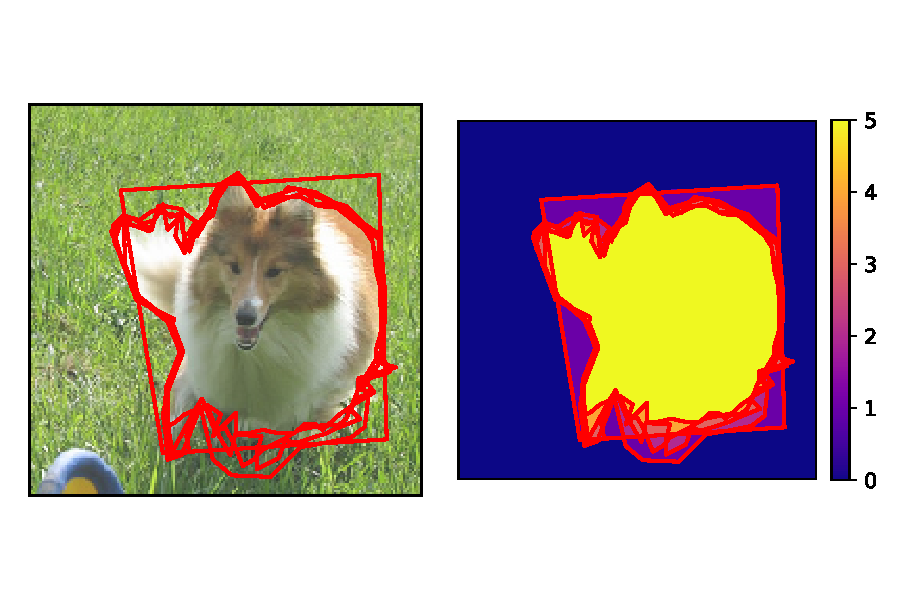
\includegraphics[width=\textwidth]{plots/tile_demo.pdf}
% \caption{Left: Red boundaries shows the segmentation boundaries drawn by five workers overlaid on the image. Right: Segmentation boundaries still shown in red. The overlaid segmentation creates a masks where the color indicates the number of workers who voted for the tile region.}
% \label{tile_demo}
% \end{figure}
At the heart of all our aggregation techniques is the ``tile'' data representation, where we logically overlay all workers' segmentations on top of each other within the framework of the overall image, as illustrated in Figure \ref{tile_demo}, to create non-overlapping discrete tile units. The intuition here is that by splitting the image into tiles, we get finer granularity information than by looking at complete segmentations. This also allows us to aggregate data from multiple workers rather than having to choose a single worker bounding box---this allows for the potential of choosing the best partial segmentations for an object and joining them, or fixing one worker's errors by taking the help of another worker's segmentation. Now, we will describe several algorithms for picking a good set of tiles.

\stitle{Aggregation: Majority Vote Aggregation (MV):} Include tiles in the output segmentation if and only if the tile is covered by at least 50\% of all worker segmentations.

\stitle{Aggregation: Expectation-Maximization (EM)}
Unlike MV, which assumes that all workers performs uniformly, EM approaches use worker quality models to infer the likelihood that a tile is part of the ground truth segmentation. An EM framework is used to simultaneously estimate both worker qualities and tile likelihoods as hidden variables. We detail the formal derivation and three worker quality models that we have developed in more detail in our technical report.

\stitle{Aggregation: Greedy Tile Picking (greedy)} Using estimated tile probabilities to estimate intersection area between ground truth and tile. Greedily pick tiles with the largest intersection area ratio until Jaccard score begins to decrease. The Jaccard score is computed between the merged output from the selected set of tiles and MV segmentation.

\stitle{Retrieval: Number of Control Points (num pts)}
Pick the worker segmentation with the largest number of control points around the segmentation boundary (i.e. most precise drawing) as the output segmentation.

\subsection{Retrieval v.s. Aggregation-based Comparison}

\stitle{Aggregation-based methods performs significantly better than retrieval-based methods}

Figure~\ref{noGT_retrieval_vs_aggregation} shows that amongst the algorithms that do not make use of ground truth information, the performance of aggregation-based algorithms (greedy, EM) exceeds the best achievable through the existing retrieval-based method (num pts) and the vision-based algorithms. 
By making use of ground truth information, the best aggregation-based algorith can achieve a close-to-perfect average Jaccard score of 0.983 as an upper bound with the 30 workers sample, far exceeding the results achievable by any single `best' worker (J=0.91 for 30 workers in Figure~\ref{GT_retrieval_vs_aggregation}). This result demonstrates that aggregation-based methods are able to achieve better performance by performing inference at the \textit{tile} granularity, which is guaranteed to be finer than any worker's segmentations. 
 \begin{figure}[h!]
   \centering
   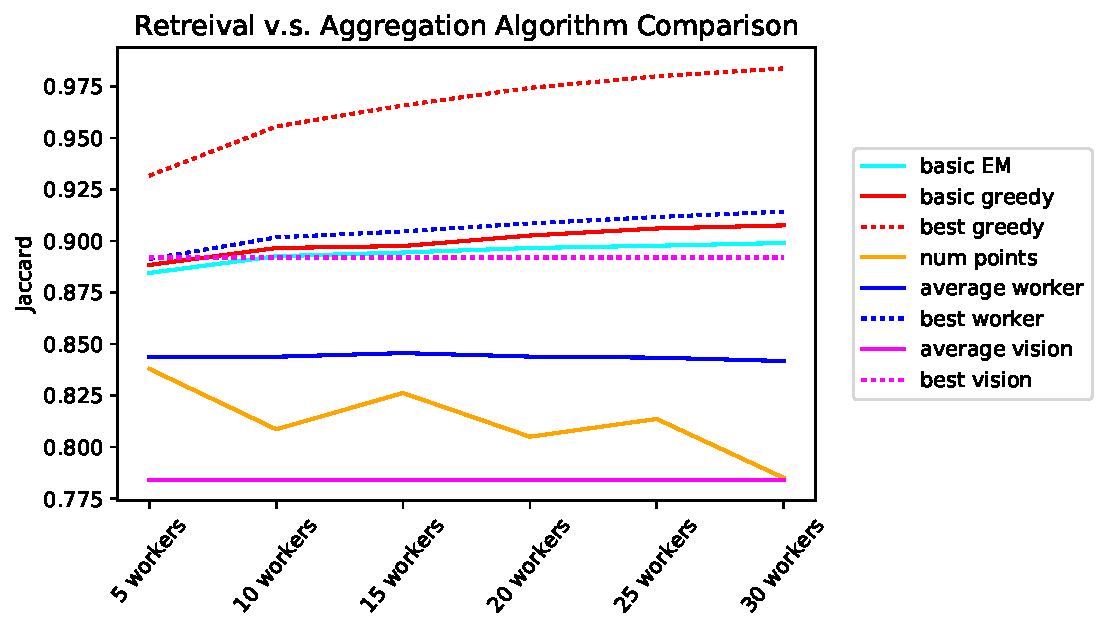
\includegraphics[width=\textwidth]{plots/Retreival_vs_Aggregation.pdf}
   \caption{Jaccard performance comparison between best-performing algorithms from retrieval and aggregation-based methods, with clustering as a preprocessing step where possible. Color denotes the type of algorithm used.}
   \label{retreival_vs_aggregation}
 \end{figure}
\dor{We should split w/ GT and no GT information into two plots side by side with same color scheme. Also consider merging greedy and EM into just one that says aggregation based method, and renaming num points as retrevial based methods.}

\stitle{Performance of aggregation-based methods scales well as more workers segmentation are added.}

Intuitively, larger worker samples results in finer granularity tiles for the aggregation-based methods, resulting in an monotonically increasing relationship between number of worker segmentation used in the sample and performance evident in Table~\ref{workerScaling}. However, worker scaling for retrieval-based methods are not guaranteed.
   \begin{table}
   \small
     \setlength\tabcolsep{1.5pt}
      \begin{tabular}{l|l|llll}
      \multicolumn{2}{c|}{Retrieval-based} & \multicolumn{4}{c}{Aggregation-based}                                                             \\ \hline
      num pts         & best worker        & \multicolumn{1}{l|}{MV}   & \multicolumn{1}{l|}{EM}   & \multicolumn{1}{l|}{greedy} & best greedy \\ \hline
      -6.30           & 2.58               & \multicolumn{1}{l|}{1.63} & \multicolumn{1}{l|}{1.64} & \multicolumn{1}{l|}{2.16}   & 5.59       
      \end{tabular}
      \caption{Percentage change in Jaccard between 5 workers samples and 30 workers sample averages.}
      \label{workerScaling}
      \vspace{-10pt}
   \end{table}